\chapter{New Algorithms for Social Recommendation}

After the first trial, we made use of the results and what we learned to come up with new algorithms for social recommendation. Again, these new algorithms each form a component of a minimization objective $Obj$ which is composed of sums of one or more objective components:

\begin{align}
\mathit{Obj} = \sum_i \lambda_i \mathit{Obj}_i
\end{align}

Again, a sigmoidal transform 
\begin{align}
\sigma(o) & = \frac{1}{1 + e^{-o}}
\end{align}
of regressor outputs $o \in \R$ is used to squash the outputs 
to the range $[0, 1]$.  
In places where the $\sigma$ transform may be optionally included, 
this is written as $[\sigma]$.  

\section{Hybrid Objective}

Because of the good performance of SVM, we decided to make use of its features $\f_{\x,\y}$  to make another linear regressor. Using $\la \cdot,\cdot \ra$ to denote an inner product, we define a weight
vector $\w \in \R^F$ such that $\la \w, \f_{\x,\y} \ra = \w^T \f_{\x,\y}$ is the prediction of the system. The objective component of linear CBF is therefore

\begin{align}
\sum_{(\x,\y) \in D} \frac{1}{2} (R_{\x,\y} - [\sigma] \w^T \f_{\x,\y})^2
\end{align}

However instead of using this linear CBF model by itself, we combine its predictions with the  Matchbox matrix factorization prediction model $[\sigma] \x^T U^T V y$, to get a hybrid objective component. The full objective component for this hybrid model is

\begin{align}
\sum_{(\x,\y) \in D} \frac{1}{2} (R_{\x,\y} - [\sigma] \w^T \f_{\x,\y} - [\sigma] \x^T U^T V y)^2
\end{align}

\section{New Social Regularizers}

\subsection{Social Spectral Regularization}
\begin{align}
\sum_{\x} & \sum_{\z \in \mathit{friends}(\x)} \frac{1}{2} S^+_{\x,\z} \| U\x - U\z \|_2^2 \nonumber \\
& = \sum_{\x} \sum_{\z \in \mathit{friends}(\x)} \frac{1}{2} S^+_{\x,\z} \| U (\x - \z) \|_2^2 \nonumber \\
& = \sum_{\x} \sum_{\z \in \mathit{friends}(\x)} \frac{1}{2} S^+_{\x,\z} (\x - \z)^T U^T U (\x - \z)
\end{align}

\subfive Note: standard spectral regularization assumes $S^+_{\x,\z} \in [0,1]$;
however we may also want to try $S_{\x,\z}$ since a negative value actively
encourages the latent spaces to oppose each other, which may be desired.

\subsection{Social Co-preference Regularization}

A crucial aspect missing from other SCF methods is that while two users may not be globally similar or opposite 
in their preferences, there may be sub-areas of their interests which can be correlated to each other.
For example, two friends may have similar interests concerning music, but 
different interests concerning politics.  The social co-preference regularizers
aim to learn such selective co-preferences. The motivation is to constrain users $\x$
and $\z$ who have similar or opposing
preferences to be similar or opposite in the same latent latent space
relevant to item $\y$.  

We use $\la \cdot, \cdot \ra_{\bullet}$ to denoe a reweighted inner product. The objective component for 
social co-preference regularization along with its expanded form is

\begin{align}
\sum_{(\x,\z,\y) \in C} & \frac{1}{2} (P_{\x,\z,\y} - \la U\x, U\z \ra_{V\y})^2 \nonumber \\
& = \sum_{(\x,\z,\y) \in C} \frac{1}{2} (P_{\x,\z,\y} - \x^T U^T \diag(V\y) U \z)^2
%= & \sum_{(\x,\z,\y) \in C}  \frac{1}{2} (P_{\x,\z,\y} - \sum_{k=1}^K (U\x)_k (U\z)_k (V\y)_k )^2 
\end{align}


\subsection{Social Co-preference Spectral Regularization}
This is the same as the social co-preference regularization above, except that it uses the spectral regularizer format for 
learning the co-preferences.

 We use $\| \cdot \|_{2,\bullet}$ to denote a re-weighted $L_2$ norm. The objective component for
 social co-preference spectral regularization along with its expanded form is
 
\begin{align}
\sum_{(\x,\z,\y) \in C} & \frac{1}{2} P_{\x,\z,\y} \| U\x - U\z \|_{2,V\y}^2 \nonumber \\
& = \sum_{(\x,\z,\y) \in C} \frac{1}{2} P_{\x,\z,\y} \| U (\x - \z) \|_{2,V\y}^2 \nonumber \\
& = \sum_{(\x,\z,\y) \in C} \frac{1}{2} P_{\x,\z,\y} (\x - \z)^T U^T \diag(V\y) U (\x - \z)
%= & \sum_{\x} \sum_{\z \neq \x} \sum_{\y} \frac{1}{2} P_{\x,\z,\y} \sum_{k=1}^K \big( \left[ (U\x)_k - (U\z)_k \right] (V\y)_k \big)^2
\end{align}

\subsection{Derivatives}
As before, we seek to optimize sums of the above objectives and will use
gradient descent for this purpose. We again use the following useful abbreviations:

\begin{align*}
\s & = U \x \qquad \s_{k} = (U \x)_{k}; \; k=1\ldots K\\
\t & = V \y \qquad \t_{k} = (V \y)_{k}; \; k=1\ldots K
\end{align*}

The derivatives for the linear CBF and hybrid objective functions, as well as the new social regularizers are
 
\begin{itemize}
\item {\bf Explicit Linear CBF}:
\begin{align*}
\frac{\partial}{\partial \w} \Obj_\pcbf & = \frac{\partial}{\partial \w} \sum_{(\x,\y) \in D} \frac{1}{2} \left( \underbrace{(R_{\x,\y} - [\sigma] \overbrace{\w^T \f_{\x,\y}}^{o_{\x,\y}})}_{\delta_{\x,\y}} \right)^2\\
& = \sum_{(\x,\y) \in D} \delta_{\x,\y} \frac{\partial}{\partial \w} - [\sigma] \w^T \f_{\x,\y}\\
& = - \sum_{(\x,\y) \in D} \delta_{\x,\y} [\sigma(o_{\x,\y}) (1 - \sigma(o_{\x,\y}))] \f_{\x,\y}
\end{align*}

\item {\bf Hybrid}:
\begin{align*}
\frac{\partial}{\partial \w} \Obj_\phy & = \frac{\partial}{\partial \w} \sum_{(\x,\y) \in D} \frac{1}{2} \left( \underbrace{R_{\x,\y} - [\sigma] \overbrace{\w^T \f_{\x,\y}}^{o^1_{\x,\y}} - [\sigma] \x^T U^T V\y}_{\delta_{\x,\y}} \right)^2 \\
& = \sum_{(\x,\y) \in D} \delta_{\x,\y} \frac{\partial}{\partial \w} - [\sigma] \w^T \f_{\x,\y} \\
& = - \sum_{(\x,\y) \in D} \delta_{\x,\y} [\sigma(o^1_{\x,\y}) (1 - \sigma(o^1_{\x,\y}))] \f_{\x,\y} 
\end{align*}
\begin{align*}
\frac{\partial}{\partial U} \Obj_\phy & = \frac{\partial}{\partial U} \sum_{(\x,\y) \in D} \frac{1}{2} \left( \underbrace{R_{\x,\y} - [\sigma] \w^T \f_{\x,\y} - [\sigma] \overbrace{\x^T U^T V\y}^{o^2_{\x,\y}}}_{\delta_{\x,\y}}\right)^2 \\
& = \sum_{(\x,\y) \in D} \delta_{\x,\y} \frac{\partial}{\partial U} - [\sigma] \x^T U^T V\y \\
& = - \sum_{(\x,\y) \in D} \delta_{\x,\y} [\sigma(o^2_{\x,\y}) (1 - \sigma(o^2_{\x,\y}))] \t \x^T\\
%\end{align*}
%\begin{align*}
\frac{\partial}{\partial V} \Obj_\phy & = \frac{\partial}{\partial V} \sum_{(\x,\y) \in D} \frac{1}{2} \left( \underbrace{R_{\x,\y} - [\sigma] \w^T \f_{\x,\y} - [\sigma] \overbrace{\x^T U^T V\y}^{o^2_{\x,\y}}}_{\delta_{\x,\y}}\right)^2 \\
& = \sum_{(\x,\y) \in D}  \delta_{\x,\y} \frac{\partial}{\partial V} - [\sigma] \x^T U^T V\y \\
& = - \sum_{(\x,\y) \in D}  \delta_{\x,\y} [\sigma(o^2_{\x,\y}) (1 - \sigma(o^2_{\x,\y}))] \s \y^T \\
\end{align*}

\item {\bf Social spectral regularization}:
\begin{align*}
\frac{\partial}{\partial U} \Obj_\rss & = \frac{\partial}{\partial U} \sum_{\x} \sum_{\z \in \mathit{friends}(\x)} \frac{1}{2} S^+_{\x,\z} (\x - \z)^T U^T U (\x - \z) \\
& = \sum_{\x} \sum_{\z \in \mathit{friends}(\x)} \frac{1}{2} S^+_{\x,\z} U ((\x - \z)(\x - \z)^T + (\x - \z)(\x - \z)^T)\\
& = \sum_{\x} \sum_{\z \in \mathit{friends}(\x)} S^+_{\x,\z} U (\x - \z)(\x - \z)^T
\end{align*}
\end{itemize}
Before we proceed to the final derivatives, we define one additional
vector abbreviation: 
\begin{align*}
\r & = U \z \qquad \r_{k} = (U \z)_{k}; \; k=1\ldots K .
\end{align*}
\begin{itemize}
\item {\bf Social co-preference regularization}:
\begin{align*}
\frac{\partial}{\partial U} \Obj_\rsc & = \frac{\partial}{\partial U} \sum_{(\x,\z,\y) \in C} \frac{1}{2} \left( \underbrace{P_{\x,\z,\y} - \x^T U^T \diag(V\y) U \z}_{\delta_{\x,\z,\y}} \right)^2\\
& = \sum_{(\x,\z,\y) \in C} \delta_{\x,\z,\y} \frac{\partial}{\partial U} - \x^T U^T \diag(V\y) U \z \\
%%%%%%%%%%%%%%%%%%%%%%%%%%%%%%%%%%%%%%%%%%%%%%%%%%%%%%%%%%%%%%%%%%%%%%%%
%& = \delta \frac{\partial}{\partial U} - \tr(\diag(\x) U^T \diag(V\y) U \diag(\z)) \\
%& = - \delta \diag(\z) \diag(\x) U^T \diag(V\y) + \diag(\x)^T \diag(\z)^T U^T \diag(V\y)^T\\
%& = - \delta \diag(V\y)^T U \diag(\x)^T \diag(\z)^T + \diag(V\y)^T U \diag(\z)^T \diag(\x)^T\\
%& = - \delta \diag(V\y)^T U (\diag(\x) \diag(\z) + \diag(\z) \diag(\x)) \\
%& = - \delta \diag(V\y)^T U (\z \x^T + \x \z^T) \\
%%%%%%%%%%%%%%%%%%%%%%%%%%%%%%%%%%%%%%%%%%%%%%%%%%%%%%%%%%%%%%%%%%%%%%%%
% Found it, see here for direct derivative: http://www.ee.ic.ac.uk/hp/staff/dmb/matrix/calculus.html
& = - \sum_{(\x,\z,\y) \in C} \delta_{\x,\z,\y} (\diag(V\y)^T U \x \z^T + \diag(V\y) U \z \x^T)\\ % \diag(V\y)^T = \diag(V\y)
& = - \sum_{(\x,\z,\y) \in C} \delta_{\x,\z,\y} \diag(V\y) U (\x \z^T + \z \x^T)\\
\end{align*}
In the following, $\circ$ is the Hadamard elementwise product:
\begin{align*}
\frac{\partial}{\partial V} \Obj_\rsc & = \frac{\partial}{\partial V} \sum_{(\x,\z,\y) \in C} \frac{1}{2} (P_{\x,\z,\y} - \x^T U^T \diag(V\y) U \z)^2\\
 & = \frac{\partial}{\partial V} \sum_{(\x,\z,\y) \in C} \frac{1}{2} \left( \underbrace{P_{\x,\z,\y} -  (\overbrace{U\x}^\s \circ \overbrace{U\z}^\r)^T V\y}_{\delta_{\x,\z,\y}} \right)^2\\
 & = \sum_{(\x,\z,\y) \in C} \delta_{\x,\z,\y} \frac{\partial}{\partial V} - (\s \circ \r)^T V\y\\
 & = - \sum_{(\x,\z,\y) \in C} \delta_{\x,\z,\y} (\s \circ \r) \y^T
\end{align*}
\item {\bf Social co-preference spectral regularization}:
\begin{align*}
\frac{\partial}{\partial U} \Obj_\rscs & = \frac{\partial}{\partial U} \sum_{(\x,\z,\y) \in C} \frac{1}{2} P_{\x,\z,\y} (\x - \z)^T U^T \diag(V\y) U (\x - \z)\\
& = \sum_{(\x,\z,\y) \in C} \frac{1}{2} P_{\x,\z,\y} \left( \diag(V\y)^T U (\x - \z) (\x - \z)^T \right.\\
& \left. \qquad \qquad \qquad \qquad + \diag(V\y) U (\x - \z) (\x - \z)^T \right)\\
& = \sum_{(\x,\z,\y) \in C} P_{\x,\z,\y} \diag(V\y) U (\x - \z) (\x - \z)^T\\
\frac{\partial}{\partial V} \Obj_\rscs & = \frac{\partial}{\partial V} \sum_{(\x,\z,\y) \in C} \frac{1}{2} P_{\x,\z,\y} (\x - \z)^T U^T \diag(V\y) U (\x - \z)\\
& = \frac{\partial}{\partial V} \sum_{(\x,\z,\y) \in C} \frac{1}{2} P_{\x,\z,\y} (U(\x-\z) \circ U(\x-\z))^T V\y\\
& = \frac{1}{2} \sum_{(\x,\z,\y) \in C} P_{\x,\z,\y} (U(\x-\z) \circ U(\x-\z)) \y^T
\end{align*}
\end{itemize}

Hence, for any choice of primary objective and one or more regularizers,
we simply add the derivatives for each of $\w$, $U$, and $V$
according to~\eqref{eq:sum_der}.

\section{Second Trial}

For the second online trial, we chose four algorithms again to randomly split between the LinkR application users. The four recommendation algorithms are:

\begin{itemize}
\item{Social Matchbox: Matchbox MF + Social Regularization +  L2 Regularization}
\item{Spectral Matchbox: Matchbox MF + Social Spectral Regularization + L2 Regularization}
\item{Social Hybrid: Hybrid + Social Regularization + L2 Regularization}
\item{Spectral Co-preference: Matchbox MF + Social Co-preference Spectral Regularization + L2 Regularization}
\end{itemize}

Social Matchbox was included again as a baseline since it was the best performing algorithm in the first trial. The other algorithms were choses as a cross-section of the different regularizers. The limit of just using four algorithms for the trials was because of the small number of users who installed the LinkR application, we felt that four algorithms was the maximum we could use and still get concrete results.

\begin{table}[h!]
\centering
\begin{tabular}{| l | c |}
\hline
{\bf Algorithm} & {\bf Users} \\
\hline
Social Matchbox & 26\\
Spectral Matchbox  & 25 \\
Spectral Co-preference & 27 \\
Social Hybrid & 25 \\
\hline
\end{tabular}
\caption{Number of Users Assigned per Algorithm.}
\end{table}

\subsection{Results}

\begin{figure}[h!]
\centering
\subfigure{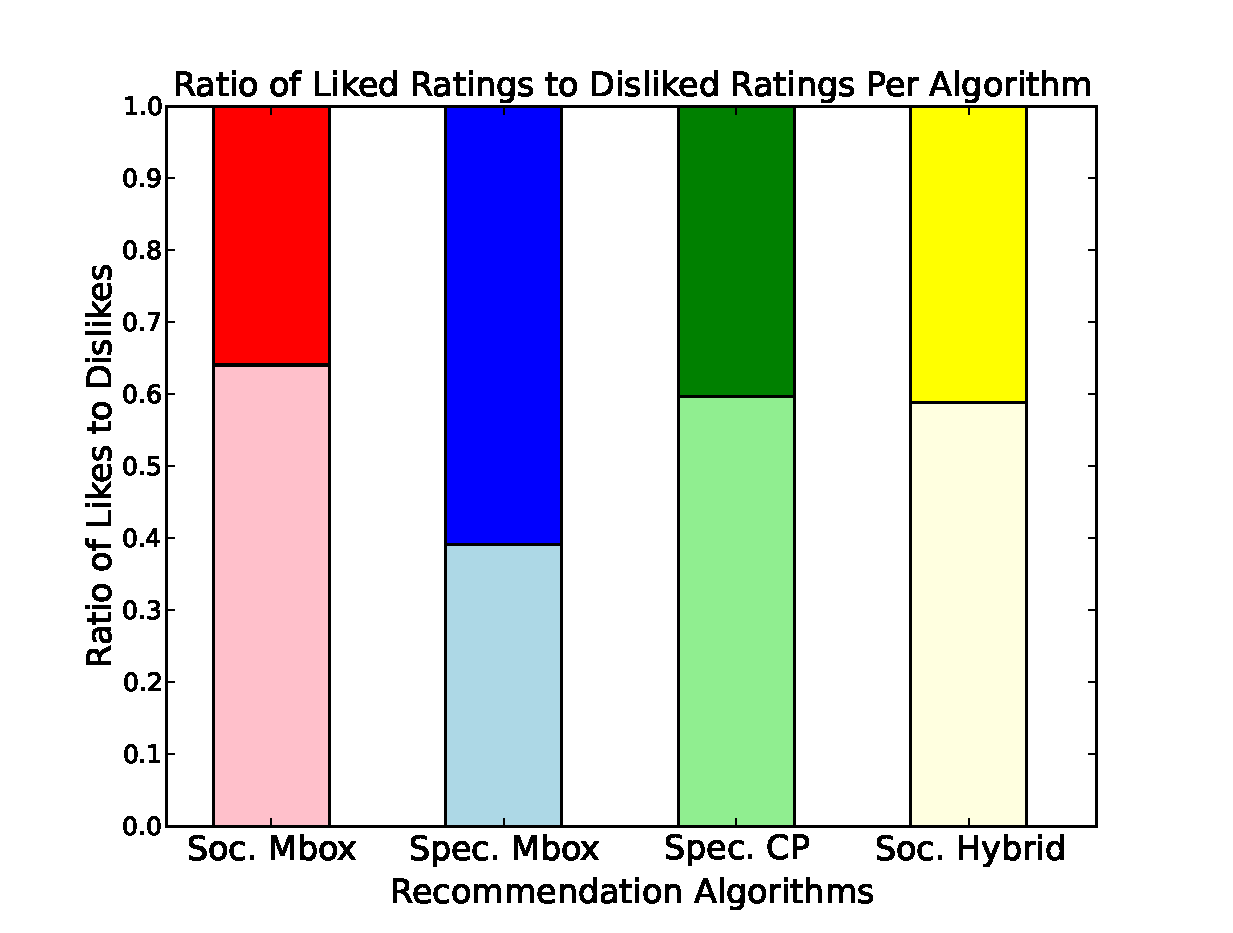
\includegraphics[scale=0.35]{img/live-likes2.eps}}
\subfigure{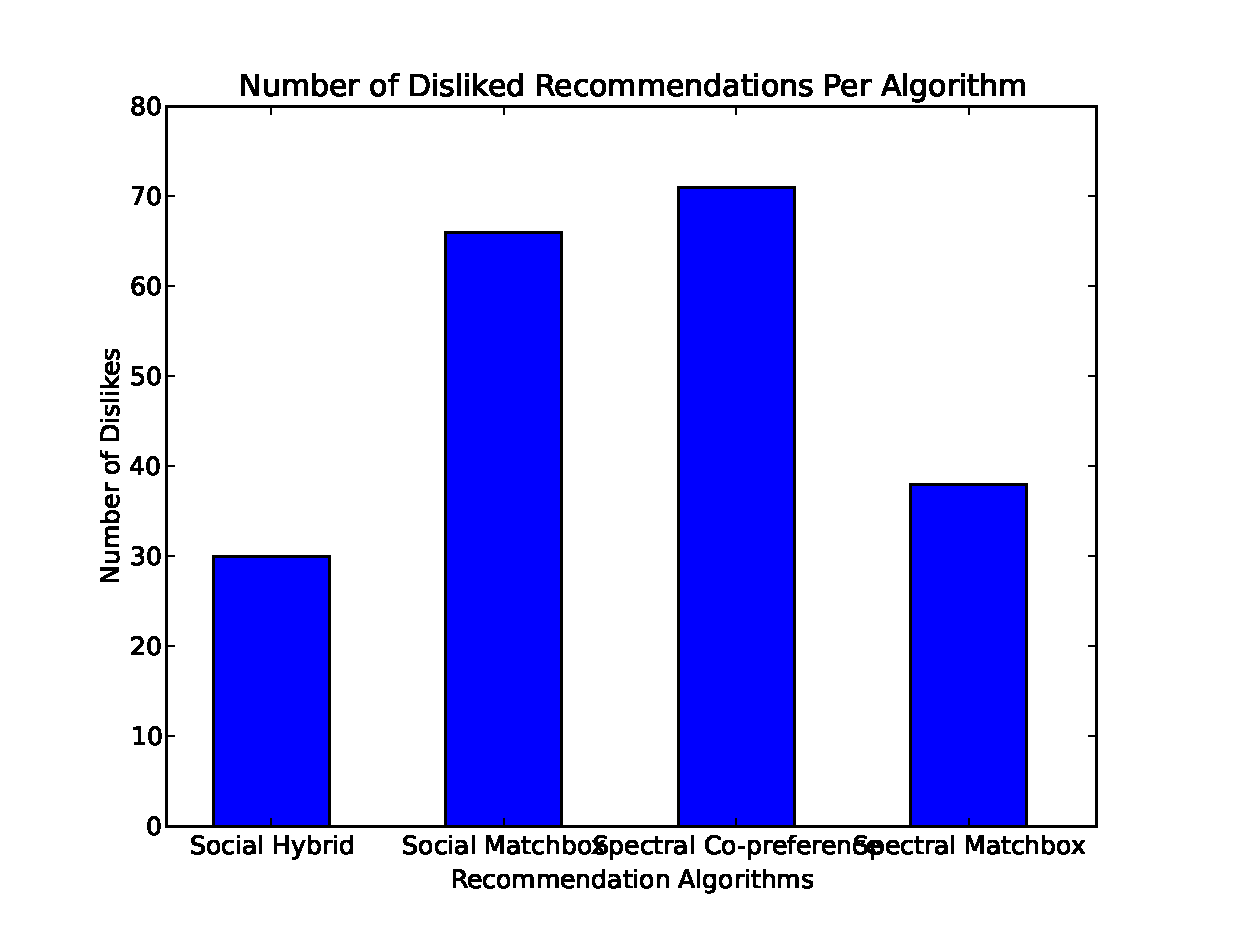
\includegraphics[scale=0.35]{img/live-dislikes2.eps}}
\caption{Results of online live trials}
\end{figure}


